%% USE one of these:
%% * the first when using pdflatex, which directly typesets your document in the
%%   chosen pdf/a format and you want to publish your thesis online,

%% * the second when you want to print your thesis to bind it, or
%% * the third when producing a ps file and a pdf/a from it.
%%
\documentclass[english, 12pt, a4paper, sci, utf8, a-1b, online]{aaltothesis}

\usepackage{graphicx}
%% Math fonts, symbols, and formatting
\usepackage{amsfonts,amssymb,amsbsy,amsmath,amsthm,enumitem,mathtools,braket,tikz}
\usepackage[capitalize]{cleveref}
\usepackage[parfill]{parskip}
\usepackage{hyphenat}
% \usepackage[style=ieee]{biblatex}
% \addbibresource{zotero.bib}

\hyphenpenalty=10000
\tolerance=1000

%% added by advisor
\usepackage{xcolor}
\newtheorem{theorem}{Theorem}
\newtheorem{lemma}[theorem]{Lemma}
\newtheorem{corollary}[theorem]{Corollary}
\theoremstyle{definition}
\newtheorem{definition}{Definition}
\theoremstyle{remark}
\newtheorem{remark}{Remark}

% advisor
\newcommand{\fda}[1]{{\color{red} \textbf{Francesco}: #1}}

% own notes
\newcommand{\TODO}{{\color{red} \textbf{TODO!} }}
\newcommand{\note}[1]{{\color{purple} \emph{#1} }}

% math commands
\newcommand{\rsquared}{{ \mathbb{R}^2 }}
% \newcommand{\nngrid}{{ n_{1}n_{2} }}
\newcommand{\nngrid}{{ n_{1}n_{2} }}

% a configuration C is a mapping ...
\newcommand{\conf}[1]{\mathcal{C}_{#1}}
% inverse of a configuration
\newcommand{\iconf}[2]{\conf{#1}^{-1}(#2)}
% normal configuration with (#2)
\newcommand{\nconf}[2]{\conf{#1}(#2)}
% text and with spacing 
\newcommand{\tand}{\text{ and }}

\newcommand{\sopt}{S_\text{opt}}

% inline math
% \DeclarePairedDelimiter{\ilmath}{\(}{\)}
\DeclarePairedDelimiter{\ilmath}{$}{$}

% euclidean norm
\DeclarePairedDelimiter{\euclnorm}{\lVert}{\rVert_2}
% manhattan norm
\DeclarePairedDelimiter{\manhattan}{\lVert}{\rVert_1}
% absolute value
\DeclarePairedDelimiter{\abs}{\lvert}{\rvert}
% set using parentheses
\DeclarePairedDelimiter{\parenset}{(\;}{\;)}




%% THESIS INFO
\degreeprogram{Computer Science}

\major{Computer Science}

\code{SCI3028.kand}

\univdegree{BSc}

\thesisauthor{Peik Etzell}

\thesistitle{Coordinated multi-robot motion planning: An overview}

\place{Espoo}

\date{\today}

\supervisor{Professor Eero Hyvönen}

\advisor{Postdoctoral researcher \\Francesco d'Amore}

\uselogo{aaltoRed}{''}

%% THE ENGLISH ABSTRACT:
%% Thesis keywords:
\keywords{}

%% The abstract text. This text is included in the metadata of the pdf file as well
%% as the abstract page.
\thesisabstract{
TODO
}

%% Copyright text. Copyright of a work is with the creator/author of the work
%% regardless of whether the copyright mark is explicitly in the work or not.
%% You may, if you wish, publish your work under a Creative Commons license (see
%% creativecommons.org), in which case the license text must be visible in the
%% work. Write here the copyright text you want. It is written into the metadata
%% of the pdf file as well.
%% Syntax:
%% \copyrigthtext{metadata text}{text visible on the page}

\copyrighttext{Copyright \noexpand\copyright\ \number\year\ \ThesisAuthor}
{Copyright \copyright{} \number\year{} \ThesisAuthor}


\begin{document}

%% Create the coverpage
\makecoverpage


%% Typeset the copyright text.
%% If you wish, you may leave out the copyright text from the human-readable
%% page of the pdf file. This may seem like a attractive idea for the printed
%% document especially if "Copyright (c) yyyy Eddie Engineer" is the only text
%% on the page. However, the recommendation is to print this copyright text.
\makecopyrightpage


%% ENGLISH ABSTRACT
%% All the details (name, title, etc.) on the abstract page appear as specified
%% above.
\begin{abstractpage}[english]
    \abstracttext{}
\end{abstractpage}

%% Force new page so that the Swedish abstract starts from a new page
\newpage

%% SWEDISH ABSTRACT.
\thesistitle{}
\supervisor{Professor Eero Hyvönen} 
\advisor{Postdoctoral researcher Francesco d'Amore}
\degreeprogram{Datateknik}
\major{Datateknik}
\keywords{}
\begin{abstractpage}[swedish]
TODO
\end{abstractpage}


% %% PREFACE
% %% This section is optional.
% \mysection{Preface}

% \vspace{5cm}
% Espoo, \today

% \vspace{5mm}
% {\hfill Peik Etzell \hspace{1cm}}

\newpage


%% TABLE OF CONTENTS
\thesistableofcontents

\clearpage

% INTRODUCTION
\section{Introduction}

% \textbf{Introduction:}
% \begin{enumerate}
%     \item broad introduction to the topic, talk about general research directions that have been investigated (be general here and cite works)
%     \item thesis objective: talk a bit more about the questions and the problems that you will address in the thesis + implication in the field
%     \item start explaining a bit more in details these topics (definitions, results, difficulties)
%     \item end of introduction: some consideration that you might have,  connections with other works, open questions (either existing or that you can come up with), etc
% \end{enumerate}

\subsection{General Overview}

Robotic motion planning is a field of research in theoretical computer science which has been deeply studied. 
It focuses on designing and studying algorithms for making robots get from one point to another safely (without colliding) and efficiently (depending on the situation, minimizing time, resource usage or similar metrics) \cite{chosetPrinciplesRobotMotion2005}.
\fda{In the last parentheses, I would just write ``minimizing some properly defined cost function''.}

Robots are modeled in a vast variety of ways, which differ in terms of shapes, sizes and kinematics: 
some warehouse robots can be modeled to move in two dimensions only, while flying drones can be seen as moving in three dimensions.

Robotic arms that move an end-effector are often modeled in six dimensions: three spatial ones and three for orientation. 
These \fda{What is ``these'' here? Not clear.} often have some so-called kinematic redundancy, meaning they have more degrees of freedom than strictly necessary. \fda{Why is the next sentence linked to the latter?}
This means that the arm is able to re-adjust while holding the same end-effector pose, which helps dexterity and fault-tolerance, but also increases complexity in planning, as poses can have different alternative joint configurations. 
\cite{sicilianoSpringerHandbookRobotics2016}
\fda{The citation goes before the period.}

There are many different environments in which robots exist. 
Assembly line robots have a fairly static environment, well defined start and end positions, and a clear and safe path between them.
Robotic vacuum cleaners on the other hand need to map their environment and make decisions dynamically, as furniture, people and pets can change places from time to time. 
Some robots need to work together; multi-robot systems can be found in warehouses \cite{sicilianoSpringerHandbookRobotics2016}, where parallel motion is highly desirable, but past research has focused mostly on algorithms moving robots one-by-one \cite{demaineCoordinatedMotionPlanning2019}.

The many real world scenarios to be studied led to the formulation of different problems.
The one we investigate in this thesis is \emph{coordinated multi-robot motion planning:} making robots move effectively without colliding with other moving robots.
The goal is to move the robots from a starting configuration to a target configuration, \fda{It seems something is missing here.}

The problem has multiple variations: \fda{after the colon we don't use capital letters I think}
In an unlabeled case \fda{I would write ``In the unlabeled version of the problem''}, we do not care which robot gets to which target position, only that all target positions get occupied. 
\fda{You can think of connecting the next sentence in a better way, such as ``If we do care about which robot reaches the target position, we are considering the \emph{labelled} version of the problem.''}
Otherwise we have a labeled problem, where robots and target positions each have labels, such that target positions contain a robot with the same label at the end. 
Note that the labels can be unique or not, and some sources \fda{What is a source? If you mean a paper, it is better to say either ``work'' or ``paper''} distinguish between these cases: for example, \cite{demaineCoordinatedMotionPlanning2019} uses \fda{``considers'' is better than ``uses''}\emph{unlabeled, colored} and \emph{labeled} as variations on the problem, such that labeled signifies unique labels \emph{it is better to specify what ``colored'' means: a reader might not know it.}

The problem can also be modeled as continuous or discrete \fda{I would say ``modeled both in the continuous or discrete space''}. The discrete variant is often handled using graph theory, while simple shapes like unit radius disks (see \cite{demaineCoordinatedMotionPlanning2019}, \cite{banyassadyUnlabeledMultiRobotMotion2022}) or unit squares (see \cite{yangCoordinatedPathPlanning2022}) are often used in the continuous case. \fda{I think continuois and discrete mean something slightly different: continuous means that you want your robots to move in a ``physical'' environment, often modeled as real Euclidean space. In this case, you have to model a robot as a unit-disk and not a point, as a point has dimension 0; in the discrete space, your ``locations'' are nodes of a graph (and not areas of the cintinuous space!!), hence the robot can be thought as occupying a whole node each time.}

Finding the minimum \emph{makespan} \fda{what does makespan mean?} solution to a discrete grid case of the problem is found to be NP-hard by \cite{demaineCoordinatedMotionPlanning2019}.
NP-hardness implies approximation algorithms are justified \cite{demaineCoordinatedMotionPlanning2019}, so research is focused on better approximations and faster computation. 

\subsection{Thesis Objective}\fda{Either you capitalize each word in each subsection, or you capitalize only the first word: compare with next subsection}

The field of coordinated motion planning for parallel robotics has seen a lot of research in recent years, with different algorithms tackling different problems in the field. 
The scope is broad and the problems are varied but related. 
The goal will be \fda{Don't use the future tense here: this IS the goal of the thesis} to understand and explain current research in the field, what has been done and what is yet to be understood.

One of the key objectives will be \fda{feels like repetitive words with respect to the previous sentence} to compare different algorithms in terms of their performance in computation and execution, strengths, weaknesses and scalability. How many robots can we support in a real system before motion planning becomes too slow? 

\subsection{Getting in depth}

\emph{TODO start explaining a bit more in details these topics (definitions, results, difficulties)}

There are two different types of motion problems: finding a collision free path from a starting configuration to a target configuration is called a \emph{motion planning problem}, while determining if such a path exists is called the \emph{mover's problem}. \cite{hopcroftReducingMultipleObject1986} 

configuration space, joint space, holonomic, obstacles, PSPACE, polynomial time in terms of what?, 

This thesis will focus on research on the motion planning problem, 

A core term is a \emph{configuration} and \emph{configuration space}.  
A configuration of a system can be modeled as a vector of all the parameters specifying the state of the system. 
In  
It lies in the configuration space of the system. 
In essence, the motion planning problem is all about finding a valid path between two distinct points in the configuration space. 

In a real world application it might be 


\subsubsection{Discrete Grid case}



\subsubsection{Continuous case}


\subsection{Considerations}

% PRELIMINARIES 
\section{Preliminaries}

\subsection{A discrete grid of robots}

% WORKSPACE 
Let our grid-based workspace be modeled as a graph \( G \coloneqq (V, E)\). 
Let it be a rectangle \(n_1 \times n_2\) where \(n_1, n_2 \geq 2 \text{ and } n_1, n_2 \in \mathbb{N}\). 
Define the vertices as \(V \coloneqq \set{1, 2, \dots , n_1} \times \set{1, 2, \dots , n_2}\).
For any \(v \in V\), let \(v_x, v_y\) be such that \(v = (v_x, v_y)\). 
We will call \(v_x\) the \(x\)-coordinate of \(v\), and \(v_y\) its \(y\)-coordinate.
To measure distance, we use the \emph{Manhattan norm} \(L_1 = \manhattan{v - w} \coloneqq (\abs{v_x - w_x} + \abs{v_y - w_y})\). Using this, the edges can be defined as \(E = \set{(v, w) \mid \manhattan{v - w} = 1 \text{ for } v, w \in V}\). In other words, nodes are only connected to their up to four immediate neighbors in the grid.

% ROBOTS AND CONFIGURATIONS
Let there be \(N \leq \nngrid\)  robots in our workspace. 
We can identify them by a number \(r \in R := \set{1, 2, \dots , N} \subset \mathbb{N}\). 
Let \(\bot\) represent the empty vertices.
A \emph{configuration} is then a mapping \(\conf{} : V \mapsto \set{1, 2, \dots, N, \bot}\) injective upon the robots in \(R\). 
Injectivity implies no two vertices in \(V\) can be occupied at once, so there will always be exactly \((\nngrid - N)\) empty squares in the grid.

% CONFIGURATION INVERSE
The \emph{inverse} of a configuration \(\iconf{}{r} = (x, y), \; r \in R\), is another function mapping robots to their respective positions.
The robots move synchronously and in parallel, up to a single edge at a time. 
A valid (no-collision) configuration \(\conf{1}\) can thus be \emph{transformed} into another valid configuration \(\conf{2}\) in a \emph{single step} if and only if:

% TRANSFORMATION REQUIREMENTS
\begin{align}
	& \parens{\iconf{1}{r} = \iconf{2}{r} \lor (\iconf{1}{r}, \iconf{2}{r}) \in E, \; \forall r \in R}\label{req:limited_movement}\\
	\land & \parens{\nconf{1}{v} = \nconf{2}{w} \Rightarrow \nconf{2}{v} \neq \nconf{1}{w}, \; \forall v, w \in V}\label{req:no_swaps}
\end{align}

In other words, \cref{req:limited_movement} means a robot can stay in place or move to a neighboring square at every step, while \cref{req:no_swaps} forbids two robots from swapping places in a single transformation step (and they can never occupy the same vertex), equivalent to a collision in the real world.

% SCHEDULE
Denote a single transformation step by \(\conf{i} \rightarrow \conf{i + 1}\). 
A \emph{schedule} is a sequence of transformation steps \(S \coloneqq \conf{1} \rightarrow \conf{2} \rightarrow \cdots \rightarrow \conf{k}\). 
A configuration \(\conf{s}\) can be transformed into a configuration \(\conf{t}\) if there exists a schedule \(\conf{s} \rightarrow \conf{s + 1} \rightarrow \cdots \rightarrow \conf{t - 1} \rightarrow \conf{t}\).

% PROBLEM DEFINITION
\begin{definition}\label{def:motion_planning_problem}
	Given a start configuration \(\conf{s}\) and a target configuration \(\conf{t}\) of a workspace, the \emph{motion planning problem} asks to find a schedule that transforms \(\conf{s}\) into \(\conf{t}\).
\end{definition}

Denote the tuple of a workspace and two configurations \(I \coloneqq \parens{G,\ \conf{s},\ \conf{t}}\) as a problem \emph{instance}. 

\begin{remark}\label{remark:reachability}
	For a \(2 \times 2\) square and any \(1 \times n\) rectangle, where \(n \geq 2\), there exist pairs of configurations that are not reachable from each other via any schedule. 
	See \cref{fig:reachability} for an example. For any other rectangular workspace there always exists such a schedule. 
\end{remark}

% IMPOSSIBLE 2*2 SQUARE FIGURE
\begin{figure}[h]
	\centering
	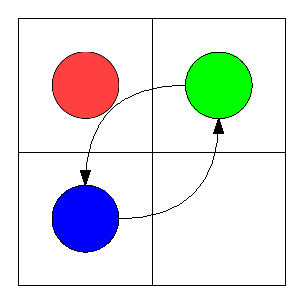
\includegraphics[width=4cm]{include/impossible_2x2.eps}
	\caption{A minimal example of an unsolvable motion planning problem: there exists no valid schedule which swaps the green and blue robots.}\label{fig:reachability}
\end{figure}

% MAKESPAN
\begin{definition}\label{def:makespan}
	The number of single transformation steps in a schedule is called the \emph{makespan} of that schedule.
\end{definition}

\begin{definition}\label{def:optimality}
	Let \(\schedules\) denote the set of all valid schedules for some problem instance \(I\). 
	A schedule \(S_\text{opt}\) is \emph{optimal} with respect to some cost function \(f : \schedules \mapsto \mathbb{N}\) mapping all valid schedules to some integer value if and only if \(f(S) \geq f(\sopt)\) for all such valid schedules \(S \in \schedules\).
\end{definition}

% M3PP -- MINIMUM MAKESPAN MOTION PLANNING PROBLEM
\begin{definition}\label{def:m3pp}
	Let the makespan of a schedule be such a cost function: \(M : S \mapsto \parens{\text{number of steps in S}}\). 
	The \emph{minimum makespan motion planning problem} asks to find an \emph{optimal} schedule with respect to the makespan \(M\) for some input problem instance.
\end{definition}

\begin{remark}
	The \emph{minimum makespan} for any motion planning problem instance \(I \coloneqq \parens{G,\ \conf{s},\ \conf{t}}\) is bounded below by \(\max(\set{\manhattan{\iconf{s}{r}, \; \iconf{t}{r}}, \; r \in R})\).
\end{remark}

\begin{definition}
	Let the aforementioned lower bound to a schedule with makespan \(M\) be denoted by \(L\). 
	The \(\emph{stretch factor}\) for that schedule is then defined as \(\frac{M}{L}\), which is always at least 1. 
\end{definition}

\subsection{Some general notation}

\begin{definition}
	A function \(f(n)\) has an asymptotic upper bound \(g(n)\) if there are some constants \(c \text{ and } n_0\) such that \(f(n) \leq c\cdot g(n),\ \forall n \geq n_0\). 
	It is then denoted as \(f(n) = \mathcal{O}(g(n))\). 
\end{definition}

% Let \emph{A} be some algorithm. 
% \fda{\(A\) is said to run in \emph{polynomial time} ... if the execution of \(A\) by a deterministic Turing machine is done in a polynomial number of steps w.r.t.\ the input bit length... (are yyou sure you want do define this? I think is better to assume it is known)}
% It is \emph{polynomial time} and often said to be \emph{efficient} if the runtime of \emph{A} is bounded by some polynomial function \(T(A) = O(n^c)\) for some constant \(c\).

Let OPT be the optimal (minimum) value of some function \(f\). 
If some algorithm \(A\) can always find a solution that maps to within a \(\rho\)-factor of the optimal value: \(OPT \leq f(x_A) \leq \rho \cdot OPT\), the algorithm is called a \(\rho\)-approximation algorithm. 


% PAPERS 
\section{The general minimum makespan parallel motion planning problem on a grid is NP-hard}

\cite{siamcomp/DemaineFKMS19} \cite{corr/YuL15c}

\subsection{Preliminaries}

\begin{definition}
	Turing machine
\end{definition}

\begin{definition}
	3SAT
\end{definition}

\subsection{The theorem}

\begin{theorem}
	The problem of computing a schedule with minimum makespan to a colored motion planning problem on a grid is NP-hard.
\end{theorem}

\begin{proof}
	\dots
\end{proof}

\section{Reconfiguration by swap operations}

\subsection{Preliminaries}

Let \ilmath{v = (x,\ y),\ w = (x,\ y)} be two nodes with \ilmath{x}- and \ilmath{y}-coordinates. Let the \emph{infinity norm} be defined as \ilmath{L_\infty = \linfty{v - w} \coloneqq \max\parens{\abs{v_x - w_x},\ \abs{v_y - w_y}}}.

Let \ilmath{d \coloneqq \max_{r \in R}\parens{\linfty{\iconf{s}{r} - \iconf{t}{r}}}}.

\subsection{Transformations by disjoint swap routines}

Given a \ilmath{2 \times 3} (or \ilmath{3 \times 2}) rectangle with up to six robots, \cite{siamcomp/DemaineFKMS19} shows that any two configurations \ilmath{\conf{1}} and \ilmath{\conf{2}} of this rectangle are within 7 transformation steps from each other. This results in a workspace being able to be subdivided into multiple of these rectangular blocks that can be independently permutable in constant time. See \cref{fig:swap3} for a visual of swapping two neighboring robots.

\cite{algorithmica/MarbergG88} introduced an algorithm called \emph{Rotatesort} which can sort an \ilmath{n_1 \times n_2} mesh in parallel in \ilmath{O(n_1 + n_2)} time. The algorithm is not built with robots in mind, and uses operations breaking the non-swapping constraint \cref{req:no_swaps} of our motion planning problem. However, with the aforementioned disjoint block division one can clearly simulate atomic swap operations in \ilmath{O(1)} time \cite{siamcomp/DemaineFKMS19}. As \ilmath{O((n_1 + n_2) \cdot O(1)) = O(n_1 + n_2)}, \cite{siamcomp/DemaineFKMS19} proves that for an \ilmath{n_1 \times n_2} workspace there is an efficient algorithm that can always compute a schedule with \ilmath{O(n_1 + n_2)} makespan.

\begin{figure}[h]
	\centering
	\includegraphics[width=0.8\linewidth]{ipe/swap3.eps}
	\caption{
		Swapping two robots in three steps using a fixed amount of space.
	}\label{fig:swap3}
\end{figure}

This clearly gives an upper bound for the optimal makespan of a parallel motion planning problem.


\subsection{Reconfiguration by utilizing subflows}

% As longer distances would ideally be traversed monotonously moving in the same direction, and not back and forth, continuously transforming \ilmath{n_1 \times n_2} rectangles, \cite{siamcomp/DemaineFKMS19} comes up with the idea of combining Rotatesort with so-called \emph{subflows}. 

Continuously transforming different subdivisions is not very efficient: it would be a lot better to be able to make robots traverse longer distances in some kind of queues or flows. Let \ilmath{d \coloneqq \max_{r \in R} \max  } \cite{siamcomp/DemaineFKMS19} 


% be  permutation of 
% \cite{siamcomp/DemaineFKMS19} details how  rectangle is permutable into any always finds that an \ilmath{n_1 \times n_2} workspace can be subdivided into 

\section{Alternative metrics to makespan}\label{chapter:alternative_metrics}

Let \ilmath{\alpha_r \coloneqq \max\set{\tau' \mid \iconf{\tau}{r} = \iconf{t}{r}\ \forall \tau \geq \tau'}} be the arrival time of \ilmath{r}, i.e. the timestep when \ilmath{r} stops moving. 
Define \ilmath{P_r \coloneqq \set{ \parens{ \iconf{i}{r},\ \iconf{i + 1}{r} } \mid \parens{ \iconf{i}{r},\ \iconf{i + 1}{r} } \in E }} to be the \emph{path} of \ilmath{r}: the sequence of steps \ilmath{r} takes in a schedule. 

Consider the following well-defined cost functions:
\begin{align*}
	% \smash and manual spacing to circumvent the larger block from \max_{r \in R}
	& \mono{Makespan} 				& \mono{(M)} && \schedules \mapsto \quad & \smash{\max_{r \in R}} \ \alpha_r 	\\[2mm] 
	& \mono{Total Arrival Time} 	& \mono{(TAT)} && \schedules \mapsto \quad & \Sigma_{r \in R} \ \alpha_r 		\\[2mm]
	& \mono{Total Distance} 		& \mono{(TD)} && \schedules \mapsto \quad & \Sigma_{r \in R} \ \abs{P_r} 		\\[2mm]
	& \mono{Maximum Distance} 		& \mono{(MD)} && \schedules \mapsto \quad & \max_{r \in R} \ \abs{P_r}
\end{align*}

% \cite{corr/YuL15c} examines all four of these on a general graph, i.e. not contrained to model a grid like in our case. An important finding is proving the decision problem statements for the respective optimization problems of the cost functions above are all NP-complete on a general graph. This importantly does \emph{not} imply the same holds for the grid case of coordinated robot motion planning, and the reduction they use is not easily convertible to the grid. It seems currently unknown if the respective decision problems to these metrics are also NP-complete on the grid similar to \cref{thm:npc}.

\cite{corr/YuL15c} finds that for a robot motion planning problem on a \emph{general} graph, one cannot always find schedules that optimize any pair of the above cost functions simultaneously: 
\begin{align}\label{eq:metric_tuple}
	\forall \parens{f_1,\ f_2} \in \set{\mono{M, TAT, TD, MD}}^2 : \exists I : \schedules_{\text{opt}_{f_1}} \cap \schedules_{\text{opt}_{f_2}} = \emptyset,
\end{align}
where \ilmath{\schedules_{\text{opt}_f} \subseteq \schedules} denotes the set of optimal schedules for an instance \ilmath{I} with respect to some cost function \ilmath{f}. 
That \cref{eq:metric_tuple} is true on a general graph does not imply that it holds for our problem formulation on a grid, and the graphs used in the proof are not compatible with our grid-model. 
However, by coming up with new grid-specific problem instances we prove the statement holds on the grid as well.

\begin{lemma}\label{lemma:simultaneous_1}
	A pairing of cost functions \ilmath{\parens{f_1, f_2} \in \set{\mono{M, MD}} \times \set{\mono{TAT, TD}}} cannot always be simultaneously optimized on the grid.
\end{lemma}

\begin{proof}

	% FIGURE SIMULTANEOUS 1 PROBLEM
	\begin{figure}[h]
		\centering
		
\includegraphics[width=0.35\linewidth]{ipe/sim1_problem.eps}
		\caption{
			A problem instance that requires different schedules depending on the cost function. Circles represent robots, crosses represent their targets. The two robots in the middle are already on their targets. 
		}
		\label{fig:sim1}
	\end{figure}

	Observe the configuration in \cref{fig:sim1}. 
	It is easy to see that there are two different ways to schedule a solution: either sacrifice maximum time and distance by letting the single robot move around the two central ones, or alternatively let the middle robots move out of the way, sacrificing the total travel time and distance instead. 
	See \cref{fig:sim1_strat} for a visual of this. 

	% FIGURE SIMULTANEOUS 1 STRATEGIES
	\begin{figure}[h]
		\centering
		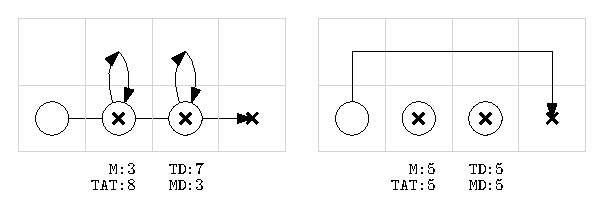
\includegraphics[width=0.7\linewidth]{ipe/sim1_strat.eps}
		\caption{
			The left schedule optimizes \mono{M}\ and \mono{MD}, while the right schedule optimizes \mono{TD}\ and \mono{TAT}.
		}
		\label{fig:sim1_strat}
	\end{figure}

It is quite trivial to conclude that there are no better solutions to this instance w.r.t. these metrics. 
This implies one cannot always optimize simultaneously for any pairing in \ilmath{\set{\mono{M, MD}} \times \set{\mono{TAT, TD}}} on the grid.
\end{proof}

\begin{lemma}\label{lemma:simultaneous_2}
	A pairing of cost functions \ilmath{\parens{f_1, f_2} \in \set{\mono{M, TAT}} \times \set{\mono{MD, TD}}} cannot always be simultaneously optimized for on the grid. 
\end{lemma}

\begin{proof}
	% FIGURE SIMULTANEOUS 2 PROBLEM
	\begin{figure}[h]
		\centering
		\includegraphics[width=0.45\linewidth]{ipe/sim2_problem.eps}
		\caption{
			A second instance that requires different schedules depending on the cost function.
		}
		\label{fig:sim2}
	\end{figure}

	% FIGURE SIMULTANEOUS 2 STRATEGIES
	\begin{figure}[h]
		\centering
		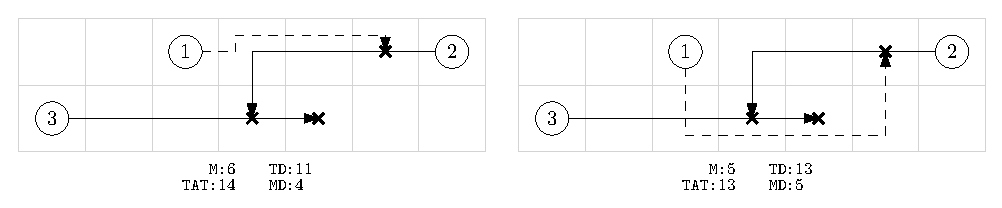
\includegraphics[width=\linewidth]{ipe/sim2_strat.eps}
		\caption{
			The left schedule optimizes \mono{TD}\ and \mono{MD}, while the right schedule optimizes \mono{M}\ and \mono{TAT}.
		}
		\label{fig:sim2_strat}
	\end{figure}

	Similarly to \cref{lemma:simultaneous_1}, observe the instance in \cref{fig:sim2}. 
	There are again two different strategies, seen in \cref{fig:sim2_strat}: robot 1 either waits for robot 2 to pass, or alternatively goes a longer distance beneath robot 2. 
	The instance is constructed so 2 and 3 have no choice but to move in these specific paths to avoid accumulating larger time and distance penalties, which means 1 has the only real choice here. 
	As there are no better schedules than these for any of these metrics, it implies no schedule exists that optimizes the specific pairs in \cref{lemma:simultaneous_2} concurrently.
\end{proof}

\begin{theorem}
	A pair of cost functions \ilmath{\parens{f_1, f_2} \in \set{\mono{M, TAT, TD, MD}}^2 } cannot always be simultaneously optimized for on the grid. 
\end{theorem}

\begin{proof}
	\begin{figure}[h]
		\centering
		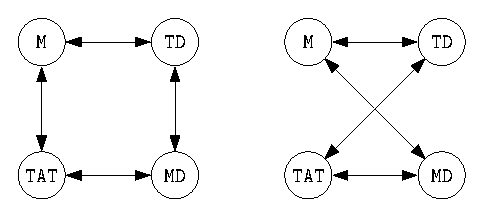
\includegraphics[width=0.5\textwidth]{ipe/sim_thm.eps}
		\caption{
			The pairs of sometimes simultaneously unoptimizable cost functions given \cref{lemma:simultaneous_1} and \cref{lemma:simultaneous_2} respectively.
		}
		\label{fig:sim_separate}
	\end{figure}

	Consider the graphs in \cref{fig:sim_separate} that show which cost functions are sometimes pairwise simultaneously unoptimizable. 
	A new graph with the same vertices and a union of the edges clearly gives us a 4-clique, which is exactly what we are after. 
	This implies the general proof from \cite{corr/YuL15c} also holds on the grid.
\end{proof}



% CONCLUSIONS
\include{chapters/conclusions.tex}

%% REFERENCES
% \bibliographystyle{aaltosci_t}
\bibliographystyle{ieeetr}
\bibliography{manual_refs}
% \bibliography{manual_refs}
% \printbibliography

\clearpage

%% ADD POSSIBLE APPENDIX HERE
\thesisappendix

\end{document}
